\documentclass{article}

\title{Sample Sweave file}
\author{Julien Arino}
\date{}

\usepackage{Sweave}
\begin{document}
\maketitle

\input{sample-RSweave-file-concordance}

The beginning of this text is automatically generated by RStudio when you create a new R Markdown file and is adapted here to Sweave. 
You can edit this text to customize the title, author, and date of the document. Sweave documents are normally rendered as PDFs.

\section*{R Sweave}

This is an R Sweave document. Sweave is a tool that allows to embed R code in a LaTeX document. 
When the document is compiled, the R code is executed and the output is included in the final document. 
This allows to create dynamic reports that automatically update when the data changes.

When you click the \textbf{Compile PDF} button, a document will be generated that includes both content as well as the output of any embedded R code chunks within the document. 
You can embed an R code chunk like this:

\begin{Schunk}
\begin{Sinput}
> summary(cars)
\end{Sinput}
\begin{Soutput}
     speed           dist       
 Min.   : 4.0   Min.   :  2.00  
 1st Qu.:12.0   1st Qu.: 26.00  
 Median :15.0   Median : 36.00  
 Mean   :15.4   Mean   : 42.98  
 3rd Qu.:19.0   3rd Qu.: 56.00  
 Max.   :25.0   Max.   :120.00  
\end{Soutput}
\end{Schunk}

\section*{Including Plots}

You can also embed plots, for example:

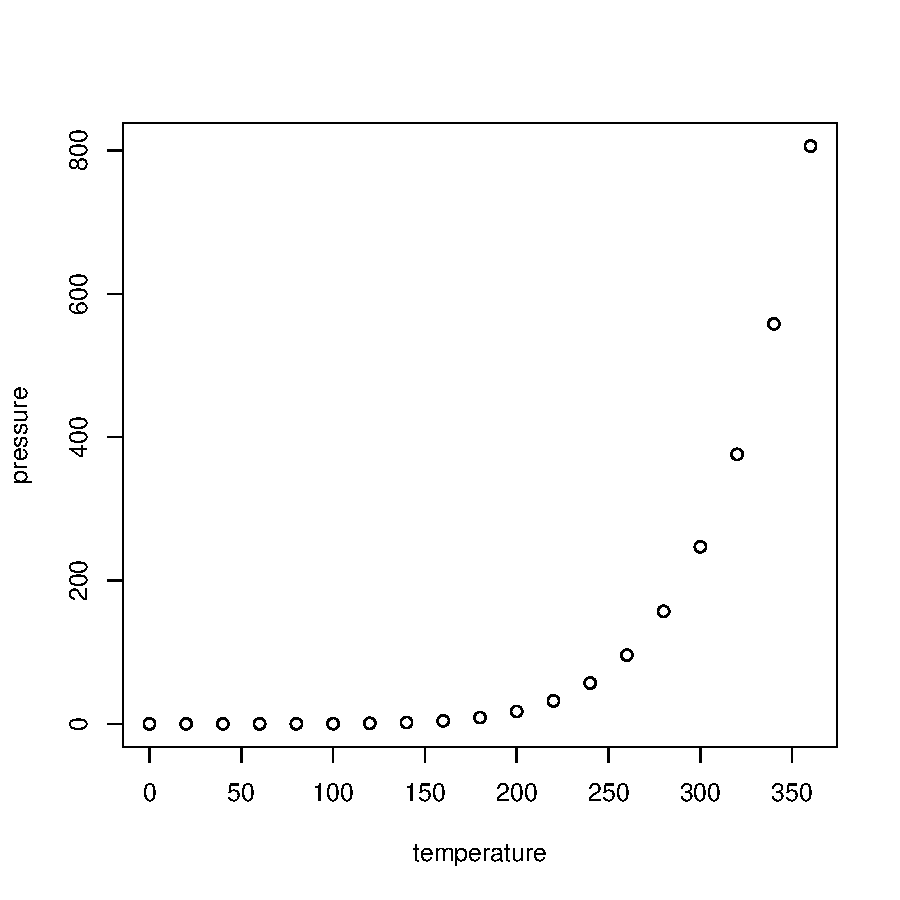
\includegraphics{sample-RSweave-file-pressure}

Note that the \texttt{echo = FALSE} parameter was added to the code chunk to prevent printing of the R code that generated the plot.

\section*{Including mathematical expressions}

\LaTeX is an advanced text language that is the go-to typesetting software in mathematics, statistics, physics and (to a large extent) computer science.
You can include mathematical expressions both inline $e^{i\pi} + 1 = 0$ and displayed:
\[
\int_{-\infty}^\infty e^{-x^2} \, dx = \sqrt{\pi}.
\]
Formatting mathematical text is done using \LaTeX syntax. 
For example, the code \verb|$e^{i\pi} + 1 = 0$| is rendered as $e^{i\pi} + 1 = 0$.

\section*{Including R code in the text}

It is also possible to include R code in the text by using the command \verb||. So I can for example write that the \texttt{cars} dataset has 50 rows and 2 columns. 

\section{One important remark: .Rmd $\neq$ .R}

This is in particular addressed to (from experience) Computer Science students: \textbf{code blocks} are not meant for you to paste your entire R code!
When marking assignments, we will be looking for a notebook feel, not just code that runs. 
This means that you should include text, explanations, and interpretations of your results as part of a coherent Sweave narrative, not stuff everything in code blocks (regardless of how much commenting of your code you do).

\subsection{Solution worth $\lim_{x \to 0} x$ marks}

\begin{Schunk}
\begin{Sinput}
> # Generate the matrix
> M = matrix(c(1,2,3,
+              4,5,6,
+              7,8,9), 
+            nrow=3, ncol=3, byrow=TRUE)
> # Compute the determinant
> det(M)
\end{Sinput}
\begin{Soutput}
[1] 6.661338e-16
\end{Soutput}
\begin{Sinput}
> # We observe that the determinant is zero (within numerical tolerance), the matrix is not invertible
\end{Sinput}
\end{Schunk}

\subsection{Solution worth a positive number of marks}
We generate the matrix
\begin{Schunk}
\begin{Sinput}
> M = matrix(c(1,2,3,
+              4,5,6,
+              7,8,9), 
+            nrow=3, ncol=3, byrow=TRUE)
\end{Sinput}
\end{Schunk}
and compute its determinant, finding det(M)=6.66133814775094e-16. We observe that the determinant is zero (within numerical tolerance), which means that the matrix is not invertible.


\end{document}
